\documentclass[border=6pt]{standalone}
% ---------------------------------------------------------------------------
% tikzpreamble.tex -- shared by main.tex and by every standalone in tikz/
% ---------------------------------------------------------------------------
\usepackage{amsmath}
\usepackage{amssymb}
\usepackage{tikz}
\usepackage{circuitikz}
\usetikzlibrary{arrows.meta,calc,positioning,decorations.pathmorphing,decorations.pathreplacing,
                decorations.markings,patterns,angles,quotes,fit,
                shapes.geometric,shapes.misc,backgrounds,intersections}

\ctikzset{bipoles/length=0.85cm}
\ctikzset{resistors/scale=0.85}
\ctikzset{capacitors/scale=0.9}

\tikzset{
  wire/.style      = {line width=0.7pt},
  dashedwire/.style= {line width=0.7pt, densely dashed},
  term/.style      = {circle, draw, line width=0.6pt, fill=white,
                      inner sep=0pt, minimum size=4.5pt},
  node dot/.style  = {circle, fill=black, inner sep=0pt, minimum size=4pt},
  boxlabel/.style  = {font=\sffamily\small},
  annot/.style     = {font=\small, align=left},
  phasor/.style    = {-{Stealth[length=3.2mm,width=2.2mm]}, line width=1.1pt},
  thinphasor/.style= {-{Stealth[length=2.6mm,width=1.8mm]}, line width=0.7pt},
  axis line/.style = {-{Stealth[length=2.6mm,width=1.8mm]}, line width=0.6pt},
  guide/.style     = {densely dashed, line width=0.4pt, gray},
}
\usepackage{siunitx}

\begin{document}
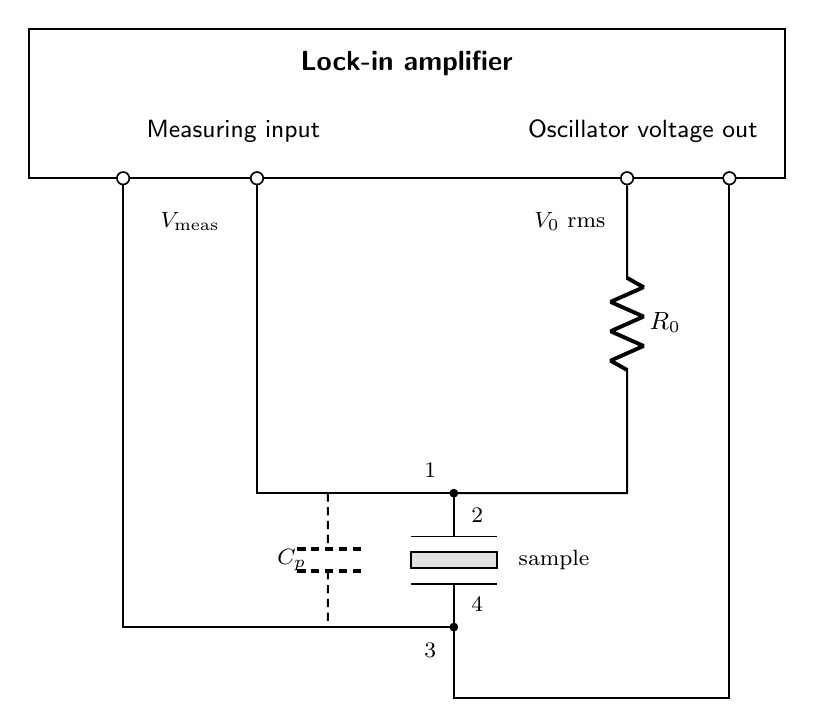
\begin{tikzpicture}[every node/.style={font=\small}]

  % ---- lock-in box -------------------------------------------------------
  \draw[wire] (0,0) rectangle (9.6,1.9);
  \node[boxlabel,font=\sffamily\bfseries] at (4.8,1.45) {Lock-in amplifier};
  \node[boxlabel] at (2.6,0.6) {Measuring input};
  \node[boxlabel] at (7.8,0.6) {Oscillator voltage out};

  \foreach \x in {1.2,2.9,7.6,8.9} { \node[term] at (\x,0) {}; }
  \node[font=\footnotesize] at (2.05,-0.55) {$V_{\mathrm{meas}}$};
  \node[font=\footnotesize,anchor=east] at (7.45,-0.55) {$V_0$ rms};

  % ---- oscillator branch through R0 -------------------------------------
  \draw[wire] (7.6,-0.09) -- (7.6,-1.1)
              to[R=$R_0$] (7.6,-2.6)
              -- (7.6,-4.0) -- (5.4,-4.0);

  % ---- sample capacitor --------------------------------------------------
  \draw[wire] (5.4,-4.0) -- (5.4,-4.55);
  \draw[wire] (4.85,-4.55) -- (5.95,-4.55);
  \draw[wire,fill=black!12] (4.85,-4.75) rectangle (5.95,-4.95);
  \draw[wire] (4.85,-5.15) -- (5.95,-5.15);
  \draw[wire] (5.4,-5.15) -- (5.4,-5.7);
  \node[node dot,minimum size=3.2pt] at (5.4,-4.0) {};
  \node[node dot,minimum size=3.2pt] at (5.4,-5.7) {};
  \node[font=\footnotesize,anchor=south east] at (5.3,-3.92) {1};
  \node[font=\footnotesize,anchor=south west] at (5.5,-4.5)  {2};
  \node[font=\footnotesize,anchor=north east] at (5.3,-5.78) {3};
  \node[font=\footnotesize,anchor=north west] at (5.5,-5.2)  {4};
  \node[font=\footnotesize,anchor=west] at (6.1,-4.85) {sample};

  % ---- return branch -----------------------------------------------------
  \draw[wire] (8.9,-0.09) -- (8.9,-6.6) -- (5.4,-6.6) -- (5.4,-5.7);

  % ---- measuring leads ---------------------------------------------------
  \draw[wire] (2.9,-0.09) -- (2.9,-4.0) -- (5.4,-4.0);
  \draw[wire] (1.2,-0.09) -- (1.2,-5.7) -- (5.4,-5.7);

  % ---- parasitic capacitance --------------------------------------------
  \draw[dashedwire] (3.8,-4.0) to[C] (3.8,-5.7);
  \node[font=\footnotesize,anchor=east] at (3.65,-4.85) {$C_p$};
\end{tikzpicture}
\end{document}
